% +------------------------------------------------------------------------+
% | Reference manual page: Apollonius_graph_data_structure_2.tex
% +------------------------------------------------------------------------+
% | 12.04.2000   Author
% | Package: Package
% | 
%\RCSdef{\RCSRegulartriangulationtraitsRev}{$Revision$}
%\RCSdefDate{\RCSRegulartriangulationtraitsDate}{$Date$}
% |
%%RefPage: end of header, begin of main body
% +------------------------------------------------------------------------+


\begin{ccRefConcept}{ApolloniusGraphDataStructure_2}

%% \ccHtmlCrossLink{}     %% add further rules for cross referencing links
%% \ccHtmlIndexC[concept]{} %% add further index entries
\ccCreationVariable{agds}
\ccDefinition

The concept \ccc{ApolloniusGraphDataStructure_2} refines the concept
\ccc{TriangulationDataStructure_2}
described in \ccRefPage{TriangulationDataStructure_2}. In addition
it provides two methods for the insertion and removal of a degree 2
vertex in the data structure. The insertion method adds a new vertex
to the specified edge, thus creating two new edges. Moreover, it
creates two new faces that have the two newly created edges in
common (see figure below). The removal method performs the reverse
operation.

\begin{figure}[htb]%\label{fig-agds-d2}
\begin{ccTexOnly}
\begin{center}
\includegraphics[width=0.8\textwidth]
{Apollonius_graph_2_ref/insert_degree_2.eps}
\end{center}
\end{ccTexOnly}
\begin{ccHtmlOnly}
<center>
<img border=0 src="./insert_degree_2.gif" align=center
alt="Insertion and removal of degree 2 vertices"
title="Insertion and removal of degree 2 vertices">
</center>
\end{ccHtmlOnly}
\begin{ccHtmlOnly}
<br><font size=-1>
\end{ccHtmlOnly}
\caption{Insertion and removal of degree 2 vertices. Left to right:
The edge \ccc{(f,i)} is replaced by two edges by means of inserting a
vertex \ccc{v} on the edge. The faces $f_1$ and $f_2$ are
created. Right to left: the faces $f_1$ and $f_2$ are
destroyed. The vertex \ccc{v} is deleted and its two adjacent edges
are merged.}
\begin{ccHtmlOnly}
</font>
\end{ccHtmlOnly}
\end{figure}



We only describe the additional requirements with respect to the
\ccc{TriangulationDataStructure_2} concept.

\ccRefines
\ccc{TriangulationDataStructure_2}

\ccHeading{Insertion}
\ccThree{Vertex_handle}{agds.insert_degree_2(Face_handle f, int i)+}{}
%
\ccMethod{Vertex_handle insert_degree_2(Face_handle f, int i);}{Inserts 
a degree two vertex and two faces adjacent to it that have two common
edges. The edge defined by the face handle \ccc{f} and the integer
\ccc{i} is duplicated. It returns a handle to the vertex created.}

\begin{ccTexOnly}
\newpage
\end{ccTexOnly}

\ccHeading{Removal}
\ccMethod{void remove_degree_2(Vertex_handle v);}{Removes a degree 2
vertex and the two faces adjacent to it. The two edges of the star of
\ccc{v} that are not incident to it are collapsed.
\ccPrecond{The degree of \ccc{v} must be equal to 2.}}


\ccHasModels
\ccc{CGAL::Apollonius_graph_data_structure_2<Vb,Fb>}

\ccSeeAlso
\ccc{TriangulationDataStructure_2}\\
\ccc{ApolloniusGraphVertexBase_2}\\
\ccc{ApolloniusGraphFaceBase_2}

\end{ccRefConcept}

% +------------------------------------------------------------------------+
%%RefPage: end of main body, begin of footer
% EOF
% +------------------------------------------------------------------------+
